\documentclass[ a4paper,
                oneside,
                toc=bibliography,
                toc=listof
                ]{scrbook}

% \usepackage[ngerman, english]{babel} % If the thesis is in English
\usepackage[english, ngerman]{babel} % If the thesis is in German


%Farbdefinitionen
\usepackage[hyperref,dvipsnames]{xcolor}

%%%
% Required for custom acronyms/glossaries style
% Left aligned Columns in tables with fixed width
% see http://tex.stackexchange.com/questions/91566/syntax-similar-to-centering-for-right-and-left
\usepackage{ragged2e}
%%%

%%%
% Abkürzungsverzeichnis
\usepackage{scrwfile} % Wichtig, ansonsten erscheint "No room for a new \write"

% von https://tex.stackexchange.com/questions/73160/table-with-tabularx-and-multirow
\usepackage{graphicx}
\usepackage{subfig}
\usepackage{tabularx}
\usepackage{multicol}
\usepackage{float}
%\setlength\columnseprule{0.5pt}

%%%
% ggf.in der Endversion komplett rausnehmen. dann auch \href in commands.tex aktivieren
% Alle Optionen nach \hypersetup verschoben, sonst crash
%
%\usepackage[]{hyperref}%siehe auch: "Praktisches LaTeX" - www.itp.uni-hannover.de/~kreutzm
%
%% Da es mit KOMA 3 und xcolor zu Problemen mit den global Options kommt MÜSSEN die Optionen so gesetzt werden.
%
%\ifdeutsch
\usepackage[ngerman]{hyperref}

% siehe http://www.dickimaw-books.com/cgi-bin/faq.cgi?action=view&categorylabel=glossaries#glsnewwriteexceeded
\usepackage[acronym,indexonlyfirst,nomain]{glossaries}
\renewcommand*{\acronymname}{Abkürzungsverzeichnis}
\renewcommand*{\glsgroupskip}{}
\makenoidxglossaries

\usepackage[ngerman,capitalise,nameinlink,noabbrev]{cleveref}
\crefname{section}{Kapitel}{Kapitel}
%\else
%\usepackage[capitalise,nameinlink,noabbrev]{cleveref}
%\fi

\usepackage[chapter]{minted}
\newmintedfile[pycode]{python}{linenos,breaklines,
               numbersep=5pt,
               frame=lines,
               framesep=2mm}
\newmintedfile[cccode]{cpp}{linenos,breaklines,
               numbersep=5pt,
               frame=lines,
               framesep=2mm}
\newmintedfile[shcode]{bash}{linenos,breaklines,
               numbersep=5pt,
               frame=lines,
               framesep=2mm}


% Eigene Farbdefinitionen ohne die Namen des xcolor packages
\definecolor{darkblue}{rgb}{0,0,.5}
\definecolor{black}{rgb}{0,0,0}

\hypersetup{
    breaklinks=true,
    bookmarksnumbered=true,
    bookmarksopen=true,
    bookmarksopenlevel=1,
    breaklinks=true,
    colorlinks=true,
    pdfstartview=Fit,
    pdfpagelayout=TwoPageRight, % zweiseitige Darstellung: ungerade Seiten rechts im PDF-Viewer - siehe auch http://tex.stackexchange.com/a/21109/9075
    filecolor=darkblue,
    urlcolor=darkblue,
    linkcolor=black,
    citecolor=black
}
%
%%%

% erweitertes Enumerate, NICHT paralist
\usepackage{enumitem}
\setlist[enumerate]{noitemsep}
\setlist[itemize]{noitemsep}
\setlist[description]{noitemsep}


% This class does the ISW styling for you (together with scrbook).
%
% It handles the following:
% - Proper input and font encoding (Just type, don't care about the LaTeX compiler you use or how to type German umlauts)
% - Fonts with ligatures and kerning (Tex Gyre fonts are used, part of every LaTeX installation, text is nice to read)
% - Bibliography styling for biblatex (declare your bibliography file and you are ready to go)
% - Provide command for title page (\makeISWtitle) and declaration of originality ( \declarationOfOriginality)
% - Loads packages "biblatex" and "graphics"
\usepackage[
    type=studie, %master, % bachelor, study, bachelorproject
]{iswthesis}

%Path to .bib-File(s) for BibLatex
\addbibresource{bibliography.bib}
\addbibresource{Studienarbeit_T3200.bib}
% \addbibresource{someOtherBibFile}
\newacronym{hil}{HIL}{Hardware-In-the-Loop}
\newacronym{imu}{IMU}{Inertial Measurement Unit}
\newacronym{uas}{UAS}{Unmanned Aircraft System}
\newacronym{uav}{UAV}{Unmanned Aerial Vehicle}
\newacronym{gps}{GPS}{Global Positioning System}
\newacronym{rpi}{RPI}{Raspberry Pi (Einplatinencomputer)}
\newacronym{tcp}{TCP}{Transmission Control Protocol}
\newacronym{udp}{UDP}{User Datagram Protocol}
\newacronym{gcs}{GCS}{Ground Control Station}
\newacronym{ram}{RAM}{Arbeitsspeicher}
\newacronym{lba}{LBA}{Luftfahrt-Bundesamt}
\newacronym{gui}{GUI}{Graphical User Interface}
\newacronym{fps}{FPS}{Frames per Second}
\newacronym{usb}{USB}{Universal Serial Bus}
\newacronym{wlan}{WLAN}{Wireless LAN}
\newacronym{uart}{UART}{Universal Asynchronous Receiver Transmitter}
\newacronym{roi}{ROI}{Region Of Interest}
\newacronym{i2c}{I\textsuperscript{2}C}{Inter-Integrated Circuit}
\newglossaryentry{csv}
{
    name=CSV,
    short={CSV},
    description={Comma Separated Values, Textdatei mit Tabelleninhalt}
}
\newglossaryentry{slam}
{
    name=SLAM,
    short={SLAM},
    description={Simultane Lokalisierung und Kartierung der Umgebung}
}
\newglossaryentry{px4}
{
    name=Pixhawk® 4,
    short=PX4,
    description={Microcontroller, mit Software und Peripherie zur Flugsteuerung}
}
\newglossaryentry{ros}
{
    name=ROS,
    short=ROS,
    description={Robot Operating System, Framework mit Schnittstellen für Sensor/Aktor-Verknüpfungen}
}
\newglossaryentry{mav}
{
    name=MAVLink,
    short=MAVLink,
    description={Binäres Übertragungsprotokoll für ressourcenbeschränkte Umgebungen, bevorzugt auf Robotern und Drohnen eingesetzt}
}


\author{Markus Rein}
\placeOfBirth{Leipzig}
\address{Alexanderstraße 146, 70180 Stuttgart}
\major{Elektrotechnik}
\title{Erweiterung bestehender Drohnen um eine Autonomflugfähigkeit}
\titleTranslated{Wie man einen Hamster trainiert}
\matrnr{6983030, TEL20GR5}
\date{21.10.22 -- 22.01.2023}
\supervisor{Prof. Dr.-Ing. Johannes Moosheimer}
\professor{Prof. Dr.-Ing. Oliver Riedel}
\usepackage{atbegshi}% http://ctan.org/pkg/atbegshi
\AtBeginDocument{\AtBeginShipoutNext{\AtBeginShipoutDiscard}} 
    
\begin{document}
    \frontmatter
    \makeISWtitle
    
    \cleardoublepage
	\setcounter{page}{1} % start at page (i) after title page
    \declarationOfOriginality

    % Kurzfassung/Abstract
    
    \cleardoublepage
    \tableofcontents

    \mainmatter

    % ********************************************************************
    % Write your own contents here:
    % ********************************************************************
    \chapter{Einführung in Projekt}
Auf physikalische Zusammenhänge wird in der Arbeit nicht eingegangen, da am bestehenden System Drohne keine Änderungen vorgenommen werden. Es wird lediglich die Software angepasst, was die Flugfähigkeit aber nicht beeinflußt.

\section{Verwendete Technologien}
\subsection{WLAN}
\subsection{GPS}

\section{Beschreibung der Drohne in den einzelnen Phasen}
\subsection{Beschreibung des Ausgangsystems Drohne}
Die Drohne kann mit Methoden der Regelungstechnik als adaptives System beschrieben werden. Dabei dient der Flugcontroller als Regler, die Motoren als Steuerstrecke, und Bordcomputer sowie Bodenstation zur Identifikation und Modifikation der Parameter. Zu Beginn wird die Drohne in ihrer Ausgangslage, ohne automone Flugfähigkeiten beschrieben. Die Bestandteile des Systems sind zunächst in Tabelle \ref{tab:system_intro} aufgelistet.

\begin{table}[!ht]
    \caption{Systemübersicht Drohne und Bodenstation}
    \begin{tabularx}{\textwidth}{l | X | X | X }
    & \multicolumn{2}{c |}{Drohne} & \\
    & Flugcontroller & Bordcomputer & Bodenstation \\ \hline
    Funktion & Autopilot-Software liest Sensoren und steuert Motoren der Drohne & Bereitstellung \acrshort{wlan}-Netzwerk zur Verbindung von Autopilot und Bodenstation & Parametrierung und Steuerung der Drohne\hfill \\ \hline
    Hardware & Pixhawk 4 & Raspberry Pi 3B+ & PC und/oder Smartphone \hfill \\ \hline
    Software & PX4 & MAVLink-Router% \newline -ROS-Umgebung \newline -Avoidance \newline Hindernisse, Trajektorie, Flugcontroller bedienen, Ultraschallsensoren
    & QGroundControl \hfill \\
    \label{tab:system_intro}
    \end{tabularx}
\end{table}

Zusammen bilden sie ein System wie in Bild \ref{fig:system_intro} gezeigt. Im Flugbetrieb werden von der Bodenstation Flugbefehle (feste Zielkoordinaten, relative Koordinaten, oder manuelle Motoransteuerung) per \acrshort{wlan}-Verbindung an den Bordcomputer, von diesem per Serieller Schnittstelle (\acrshort{uart}) an den Flugcontroller, geschickt. Mehr Details zur Steuerung mit der Bodenstation in \cref{chap:intro_capabilities}. Der Flugcontroller steuert anschließend die Motoren um die gewünschte Position zu erreichen. Als Eingabegrößen stehen dem Flugcontroller Sensordaten von Beschleunigungssensor, Kompass (erstere bilden zusammen die \gls{imu}) und Barometer, diese sind im Flugcontroller integriert, und der GPS-Antenne zur Verfügung.

\subsection{Beschreibung des Zielsystem Drohne mit autonomer Flugfähigkeit}
Zusätzliche Sensoren stellen Daten für Berechnungen auf dem Bordcomputer bereit. Diese müssen ausgewertet und die Ergebnisse dem Flugcontroller zugespielt werden. Das Auswerten und Zuspielen der Daten ist zeitkritisch denn es beeinflußt direkt den Flug der Drohne. Im Idealfall sollten Berechnungen direkt auf dem Flugcontroller oder in unmittelbarem Zusammenhang mit diesem durchgeführt werden. Zu den Aufgaben zählt:
\begin{itemize}
    \item Erfassen von Ultraschall-Daten zum Detektieren von Hindernissen
    \item Erfassen von Bildern
    \item Verarbeiten von Bildern zur Detektieren von Hindernissen
    \item Berechnung alternativer Flugbahn zur Umgehung von Hindernissen
\end{itemize}

Die Umsetzung der Flugplanung soll mittels der Software \textit{Avoidance} erfolgen. Diese arbeitet auf dem Metabetriebssystem \acrshort{ros}, welches wiederum auf \textit{Ubuntu} aufsetzt. (Im Anwendungsfall ROS Noetic auf Ubuntu 20.04.) Die Software kann vollständig auf dem \gls{rpi} betrieben werden. Somit ergeben sich für den \gls{rpi} weitere Aufgabenbereiche, wie nachfolgend dargestellt. Das erweiterte System ist dargestellt in Bild \ref{fig:system_added_sensors}.

\begin{itemize}
    \item Ubuntu 20.04 als Betriebssystem (nur indirekt möglich innerhalb eines Containers möglich)
    \item \acrshort{ros}-Noetic innerhalb des Docker-Containers
    \item Einlesen der Ultraschallsensordaten, erzeugen von Tiefenkarte und publizieren entsprechender Topic
    \item Einlesen der Kamerabilder, erzeugen von Tiefenkarte und publizieren entsprechender Topic
    \item Ausführung von Avoidance
\end{itemize}

\subsection{Beschreibung der Simulation}\label{chap:intro_simulation}
Die Entwicklung von Software für und im Zusammenhang mit dem Flugcontroller sieht vor, in einer Simulation getestet zu werden. Von der Dronecode-Stiftung wird als offizielle Umgebung dazu der Simulator \textit{Gazebo} empfohlen\cite{dronecodestiftungSimulationPX4User}. Sowohl die \textit{PX4}- als die \textit{Avoidance}-Software können vollständig in diesem betrieben werden. Zum Betrieb des Simulators wird wieder das Betriebssystem Linux Ubuntu benötigt. Deshalb werden für das Projekt einige Einschränkungen aufgenommen. Die weiteren Ausführungen hier beschreiben die Ausgangslage zur Simulation, in \cref{chap:intro_avoidance} wird \acrshort{ros} eingeführt und eingerichtet.

Zum Vorgehen wird der \gls{hil}-Aufbau mit dem Simulator \textit{AirSim} von Microsoft\cite{microsoftcorporationWelcomeAirSim2023}, wie in \cite[Kapitel 3.4.1]{markusreinErweiterungBestehenderDrohnen2023} beschrieben, verwendet. Bild \ref{fig:system_sim} zeigt, in Anlehnung an Bild \ref{fig:system_intro}, die durch die Simulation übernommenen Funktionen. Die Komponenten sind im Betrieb wie folgt verbunden:
\begin{description}
    \item[PC-Flugcontroller:] \acrshort{usb}-Kabel, wird von \textit{AirSim} zur direkten Kommunikation mit dem Flugcontroller verwendet
    \item[PC-Bordcomputer:] \acrshort{wlan}, erlaubt Verbindung Bodenstation mit Flugcontroller
\end{description}

Die Aufgaben der Komponenten während der Entwicklung sind:
\begin{description}
    \item[Simulation:] In der Simulation werden sowohl alle physikalischen Effekte berechnet als auch die virtuelle Umgebung der Drohne dargestellt. Die Sensordaten werden der Drohne direkt von der Simulation eingespeist. Eine resultierende Ansteuerung der Motoren wird in die Simulation übernommen. Somit kann sich die Drohne in der Simulation wie in realer Umgebung bewegen. Außerdem werden von der Drohne aufgenommene, simulierte Kamerabilder bereitgestellt.
    \item[Drohne:] Der Flugcontroller auf der Drohne wird im \gls{hil}-Modus betrieben. Alle Ein- und Ausgänge zum Controller werden durch virtuelle Schnittstellen der Simulation ersetzt. Die Kommunikation mit dem Bordcomputer bleibt dieselbe wie zuvor, sodass die Drohne per Bodenstation gesteuert werden kann.
    \item[Bordcomputer:] Wird weiterhin nur zur Kommunikation zwischen Bodenstation und Flugcontroller verwendet. Erweiterte Funktionen werden auf einem separaten Rechner entwickelt und getestet um anschließend auf den Bordcomputer überspielt zu werden.
\end{description}

%\paragraph*{}
%Erweiterte Funktionalität wird auf dem Entwicklungsrechner in Containern, in Verbindung mit der Simulation, erprobt. Derartige fertige Anwendungen können dann direkt auf dem Bordcomputer eingesetzt werden. Bestandteile der Software sind:
%\paragraph*{}
%\begin{description}
%    \item[\gls{ros}] 
%    \item[\textit{mavros}:] auf gleicher Ebene angesiedelt wie eine Bodenstation, erlaubt Protokollübersetzung zwischen \gls{mav}- und \acrshort{ros}-Nachrichten für \acrshort{ros}-internen Datenaustausch, empfängt Daten der Drohne und sendet neue Anweisungen zur Drohne
%    \item[Tiefenverarbeitung:] arbeitet direk mit Tiefenbildern aus dem Simulator um eine \enquote{Punktwolke der Umgebung} zu generieren
%    \item[\textit{Avoidance}:] setzt neue Zielpunkte für Drohne anhand von Sensordaten der Drohne und Punktwolke von Kamera
%    \item[\textit{AirSim-Wrapper}:] nicht für Endanwendung benötigt, kommuniziert direkt mit dem Simulationsprogramm und stellt Tiefenbild bereit
%\end{description}
%
%
    \chapter{Stand der Technik}
In diesem Kapitel werden die Grundlagen verwendeter Software erläutert.
\section{Erweiterte Flugmodi der Drohne}\label{chap:intro_capabilities}
Bei Verwendung der Drohne in Verbindung mit einer Bodenstation, wird die aktuelle Position auf einer Karte eingezeichnet. Von diesem Punkt aus kann der Drohne eine Wegvorgabe eingespielt werden, der \enquote{Mission-Mode}. Dabei enthält die Karte Informationen zur ungefähren Beschaffenheit der Umgebung, sodass die Drohne nicht Tiefer fliegen würde als der Boden der Karte. Gleichzeitig sind die standardmäßigen Sicherheitsmaßnahmen eingestellt, bspw. eine Mindesflughöhe von $4m$ einzuhalten. Neben der Wegvorgabe können dem Flugcontroller weiterhin verbotene Zonen mitgeteilt werden, die nicht durchflogen werden dürfen, genannt \textit{\enquote{Geo-Fence}}. Der Algorithmus sieht derartige Zonen als Hindernis an. Bei Kontakt mit ihnen wird ein Failsafe ausgelöst. \textit{PX4} kennt zwei derartige Modi:
\begin{description}
    \item[Failsafe GeoFence:] Ein Zylinder dessen Durchmesser von der Funkreichweite der Fernbedienung und maximaler Flughöhe beschränkt ist. Bei Durchbruch verfällt die Drohne standardmäßig in den \enquote{Return-Mode} und kehrt zu ihrer Ausgangsposition zurück.
    \item[GeoFence Plan:] Kreise oder Polygone auf Karte die nicht durchflogen oder verlassen werden dürfen (je nach Einstellung). Bei Bruch der Bedingung verfällt die Drohne in den \enquote{Hold-Mode} und bleibt schlicht stehen.
\end{description}

Es ist also bereits mit Bordmitteln möglich das Flugverhalten zu beeinflussen. Für das Vorgehen mit \textit{Avoidance} kommt der \enquote{Offboard-Mode} zum Einsatz. In diesem Modus werden dem Flugcontroller ständig neue Anweisungen, als nächster Wegpunkt, eingespeist.

Weiterhin können der Drohne im Missionsmodus sogennante \gls{roi} mitgeteilt werden. Ist eine Kamera an der Drohne vorhanden, wird diese gezielt auf die Positionen gerichtet. Ist keine Kamera explizit definiert richtet sich die Drohne mit dem Bug in Richtung der \gls{roi} aus. Da die Drohne sowohl vorwärts als auch seitwärts fliegen kann, hält sie durchgehend auf den Punkt zu.

\section{ROS und Avoidance}
Das Projekt \enquote{Obstacle Detection and Avoidance}\cite{dronecodestiftungObstacleDetectionAvoidance2023}, auf GitHub verfügbar als PX4-Avoidance\footnote{\label{note1}\url{https://github.com/PX4/PX4-Avoidance}}, hier nur \textit{Avoidance} genannt, entstand in enger Zusammenarbeit mit der Dronecode Stiftung an der ETH Zürich, dem Ursprungsort aller \textit{PX4}-Software. Es arbeitet innerhalb einer \acrshort{ros}-Umgebung.

Es stehen im Projekt 3 Algorithmen zur Verfügung, die unabhängig voneinander zu betrachten sind. Alle dienen der Anpassung der Flugbahn in unbekannter Umgebung:
\begin{description}
    \item[Local Planner:] Navigiert um Hindernisse in der direkten Umgebung
    \item[Global Planner:] Speichert nahezu vollständige Karte der Umgebung und erlaubt Navigation durch Labyrinth-artige Umgebung
    \item[Safe Landing Planner:]
\end{description}

Die Software von \textit{Avoidance} erhält die Daten des Flugcontrollers über das Zwischenprogramm \textit{mavros} (\acrshort{mav}-zu-\acrshort{ros}-Übersetzung, siehe \cite[Kapitel 5.2/5.4]{markusreinErweiterungBestehenderDrohnen2023}). Es sind die Soll-Trajektorie und Sensordaten vom Flugcontroller bekannt. Außerdem wird zur Navigation eine \textit{Punktwolke} (siehe \cref*{chap:intro_pointcloud}) der Umgebung eingespeist. Falls das Programm ein Hindernis in der Flugbahn erkennt, wird eine angepasste Trajektorie an den Flugcontroller ausgegeben.

Die Software kann nicht direkt auf dem Flugcontroller ausgeführt werden, da die Berechnungen sehr viele Ressourcen (Rechenkapazität, Speicher) benötigen. Weiterhin empfehlen die Entwickler, zuerst den Local Planner zu implementieren, da dieser am besten funktioniert. Offizielle Empfehlungen der Entwickler verwenden leisstungsstarke Hardware wie Nvidia Jetson (Hardware-Unterstützung für Bildverarbeitung) oder Intel RealSense (Kamera mit Tiefenerkennung).

Im Zusammenhang mit der Software sind letztere bereits erprobt. Aufgrund des hohen Preises können sie nicht in diesem Projekt verwendet werden, siehe \cite[Kapitel 4.3.8]{wirthErweiterungBestehendenDrohne2022}. Als Alternative können auch Stereokameras verwendet werden. Beispielcode zur Einbindung von Tiefenbildern ist unter Github (siehe \cref{note1}) vorhanden. 

%Stereokamera liefert genaue Karte der Umgebung, ähnlich einem Lidar.
%Andere Methoden arbeiten eventuell nicht mit Avoidance zusammen. Doch doch

\section{Hinderniserkennung und ROS Punktwolken}\label{chap:intro_pointcloud}
Als Verschiedene Prinzipien stehen zur Hinderniserkennung zur Verfügung. Als Eingabegröße für \textit{Avoidance} müssen die verarbeiteten Bilder im Punktwolkenformat als \acrshort{ros}-Topic vorliegen.
%Quellen nicht eindeutig
%Der Fokus dieses Projektes, das Erkennen und Ausweichen von Hindernissen wird \enquote{Obstacle Avoidance} genannt. Es ist nicht zu verwechseln mit \enquote{Obstacle Detection}, dem Erkennen und Klassifizieren von Bildinhalten.
Nachfolgend vorgestellt werden die grundlegenden Techniken der Bilderkennung. 
\subsection{SLAM Algorithmus}\label{chap:slam}
\Gls{slam} Techniken entstanden bereits in den 1980-1990 Jahren und werden bspw. bei Robotern eingesetzt, die in Hallen navigieren (für die kein \acrshort{gps} verfügbar ist). Zum Einsatz kommen Kamerasysteme in Verbindung mit Entfernungssensoren (Sonar, Radar, Lidar). Die Ergebnisse von \gls{slam} können nicht garantiert werden und sind nicht reproduzierbar, weshalb es in keinen kritischen Umgebungen (bspw. wenn Verletzungsrisiko besteht) eingesetzt werden kann.

Allgemein wird \gls{slam} durch einen modularen Prozess beschrieben:
\begin{description}
    \item[Lokalisierung:] per Motorfortschritt, \gls{imu}, Kamera, etc.%\newline Bei v\gls{slam} kommen folgende Prinzipien zum Einsatz:
    \item[Kartengenerierung:] durch einen der Algorithmen
\begin{itemize}
    \item Markov-Lokalisierung: Wahrscheinlichkeit des Aufenthaltsortes wird angenommen und über Zeit verfeinert; Iterativ; Ressourcenaufwendig
	\item Kalman-Filter: Ermöglicht basierend auf Sensordaten schnelles wiederfinden aktueller Position; anfällig bei Verlust von Eingangsdaten
	\item Monte-Carlo-Lokalisierung (Partikelfilter): nimmt Wahrscheinlichkeiten für jeden Ort an; genauer als Markov-Filter; lineare Komplexität; Weniger Speicher als Kalman-Filter; Nachteil: Stillstand ohne sich ändernde Sensordaten
\end{itemize}
    \item[Messung:] per Reichweite, Marker in Umgebung
\end{description}
%was sollte hier noch hin

\paragraph*{Visual SLAM,}kurz vSLAM, stellt eine Unterform des \gls{slam} dar, bei der ausschließlich Kameras zur Erfassung der Umgebung eingesetzt werden. Algorithmen verwenden zumeist zusätzlich die Daten der \acrshort{imu}, um die Bewegung der Kamera in die Berechnung der Position einzubeziehen.

\subsection{Stereokamera}\label{chap:stereovision}
Verwendet mehrere Kameras aus parallelverschobenen Bildern Tiefeninformationen zu gewinnen. also Abstand zu Punkten im Bild zu erkennen.
\subsection{Optical Flow}
In Bewegungsabläufen werden Objekten verfolgt und können somit relativ zur Kamera bestimmt werden. Das Prinzip wird auch von Lebewesen im Gehirn angewandt. Dabei kann schlecht zwischen der Bewegung der Kamera und der Bewegung von Objekten unterschieden werden. Ungenau, da Kameras immer eine Verzerrung besitzen. 

\subsection{Punktwolkenformat}
Die Möglichkeiten Optical Flow und Stereokamera erzeugen jeweils Tiefenkarten. In diesen Bildern sind, zumeist als Graustufen, Pixel je nach Entfernung zur Kamera gekennzeichnet. Zur Umwandlung als Punktwolke muss jedes Pixel abgetastet werden um als Koordinate im 3D-Raum dargestellt werden zu können. Das \acrshort{ros} beinhaltet sowohl Progamme zur Stereoverarbeitung basierend auf OpenGL\footnote{siehe \url{http://wiki.ros.org/stereo_image_proc}}, als auch die Erzeugung von Punktwolken\footnote{siehe \url{http://wiki.ros.org/depth_image_proc}}.

    \chapter{Vorbereitung zur Umsetzung von Avoidance}\label{chap:intro_avoidance}

Um die Avoidance-Software umzusetzen, wird diese vorher in verschiedenen Modi erprobt. Dazu zählt eine Simulation. Aus dieser können die Strukturen zum Einsatz mit realer Hardware übernommen werden. Als Zwischenschritt wird die \gls{hil}-Simulation aus dem vorhergehenden Projektteil überarbeitet.

\section{Avoidance als Simulation in Software}\label{chap:sim_gazebo}
Das Avoidance-Modul arbeitet eng mit der Simulationssoftware \enquote{Gazebo} zusammen. In der Dokumentation \cite{dronecodestiftungObstacleDetectionAvoidance2023} ist die Simulation umfangreich dokumentiert, die Umsetzung des Projektes auf reale Hardware jedoch kurz gehalten.\\
Ein vollständiges Linux Ubuntu 20.04 wird benötigt, um die Software per Simulation verwenden zu können. Die Installation beinhaltet eine komplette \acrshort{ros}-Distribution mit graphischen Tools. Mithilfe mehrerer, sich gegenseitig aufrufenden, \enquote{Launch-Files} wird die Simulation instrumentiert und, aufeinander abgestimmt, gestartet. Ohne weiteres Zutun muss nur das Hauptscript zur jeweiligen Simulation aufgerufen werden. Folgend aufgelistet die vier primären Software Bestandteile:
\begin{description}
    \item[Simulator:] \textit{Gazebo}, erzeugt virtuelle Umgebung in der sich eine simulierte Drohne befindet, kann direkt mit dem Flugcontroller kommunizieren
    \item[Flugcontroller:] PX4-Flightstack, Software zur Steuerung einer Drohne, ohne echte Hardware wird ein Flugcontroller simuliert der eine Konsole und Netzwerkanbindungspunkte (via \acrshort{mav}) bereitstellt
    \item[mavros:] \acrshort{mav}-zu-\acrshort{ros}-Übersetzung, siehe \cite[Kapitel 5.2]{markusreinErweiterungBestehenderDrohnen2023}
    \item[Avoidance:] Je nach gewähltem Programm wird der \textit{Local Planner}, \textit{Global Planner}, oder \textit{Safe Landing Planner} gestartet. In diesem Projekt wird der \textit{Local Planner} erprobt.
\end{description}
Zusätzliche Programme, die beim Ausführen des \textit{Local Planner} gestartet werden, sind:
\begin{description}
    \item[rqt-reconfigure:] Feineinstellungen zum Algorithmus \textit{Local Planner} (bspw. bevorzugte Richtungskorrektur, minimale Größe erkannter Hindernisse)
    \item[rviz:] Visualisierung der Drohne im 3-Dimensionalen Raum, dargestellt wird Position der Drohne, ihres Ursprungs, Zielposition, geplante Flugroute, Punktwolkendarstellung von Hindernis, eventuell Blaupause von Hindernis (Abhängig von gewählter Umgebung)
\end{description}
Für die Untersuchung der gegebenen Situation wird zusätzliche Software verwendet:
\begin{description}
    \item[topic-explorer:] Detaillierte Informationen zu Nachrichten im \acrshort{ros}-Umfeld
    \item[tftree:] Verknüpfungen im Transformationsbaum zur Bestimmung der Position der Drohne und derer Peripherie im Bezug zum Ursprung 
\end{description}

Die Interaktion der Bestandteile ist in Abbildung \ref{fig:system_sim_origin} noch einmal dargestellt. Auf rechter Seite gezeichnet sind die Bestandteile in der \enquote{\acrshort{ros}-Umgebung}, welche in die Endanwendung übernommen werden können. Die vollen Aufgaben des Simulators wurden eingekürzt, sie sind zu lesen in \cref{chap:intro_simulation} und \cite[Kapitel 3.4.1]{markusreinErweiterungBestehenderDrohnen2023}. Zusätzlich stellt der Simulator Kamerabilder bereit, je nach gewähltem Modus direkt Tiefenbilder oder Stereobilder welche weiter verarbeitet werden müssen. 
\begin{figure}[!ht]
    \centering
    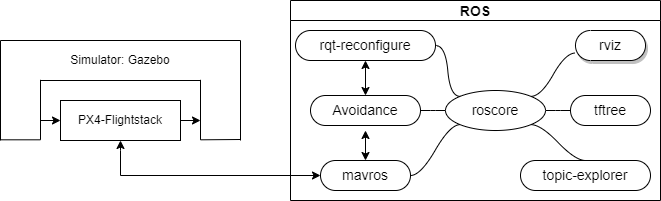
\includegraphics[width=\linewidth]{images/simulation_ros.drawio.png}
    \caption[Systemaufbau der Simulation von Avoidance als Software-Simulation]{Systemaufbau der Simulation von Avoidance als Software-Simulatio: Links Simulator (Gazebo) und Flugcontroller (reine Software), Rechts Bestandteile des \acrshort{ros}}
    \label{fig:system_sim_origin}
\end{figure}

Eine erste Überprüfung des Algorithmus wird die Simulation wie in der Anleitung\footnote{\url{https://github.com/PX4/PX4-Avoidance}\cite{dronecodestiftungObstacleDetectionAvoidance2023}} beschrieben durchgeführt. Einige Paramameter wurden zur besseren Übersichtlichkeit angepasst, sodass:
\begin{itemize}
    \item \textit{Gazebo} mit graphischer Oberfläche startet
    \item Die korrekte Punktwolken-Topic vom \textit{Local Planner} abonniert wird
    \item Die Punktwolke der Kamerabilder noch einmal gefiltert wird
\end{itemize} 

Die Anfangsbedingungen der Simulation sind eine vor Bäumen stehende Drohne. Das Bild aus der Simulation ist abgedruckt im Anhang unter \ref{fig:sim_gazebo}. Von der Drohne werden 2 virtuelle Kamerabilder erzeugt, aus welchen eine Punktwolke gebildet wird. Die Punktwolke ist in Bild \ref{fig:sim_gazebo_stereo} links dargestellt. Der Algorithmus zur Erzeugung der Punktwolke ist anfällig für Rauschen verursacht durch minimale Bewegungen in den Kamerabildern, sodass im Bild Artefakte enthalten sind. Deshalb wurde die Punktwolke noch einmal mit einem VoxelGrid\footnote{\url{http://wiki.ros.org/pcl_ros/Tutorials/VoxelGrid\%20filtering}\cite{openroboticsDocumentationROSWiki}} gefiltert, abgebildet in \ref{fig:sim_gazebo_stereo} rechts. Für die Verwendung der Punktwolke mit Avoidance macht das Filtern keine Auswirkung, der \textit{Local Planner} kommt auch mit den ursrpünglichen Daten der Punktwolke zurecht.

\begin{figure}[!ht]
    \centering
    \subfloat[][Erzeugte Punktwolke]{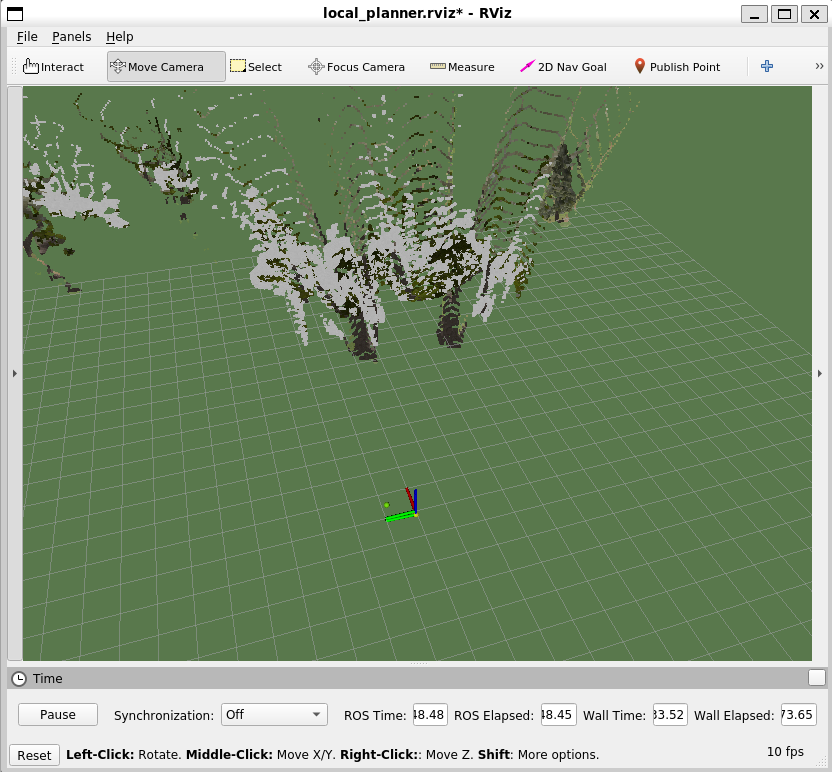
\includegraphics[width=0.4\textwidth]{images/sim_gazebo_points_stereo.png}}\hfill
    \subfloat[][Erzeugte Punktwolke, gefiltert]{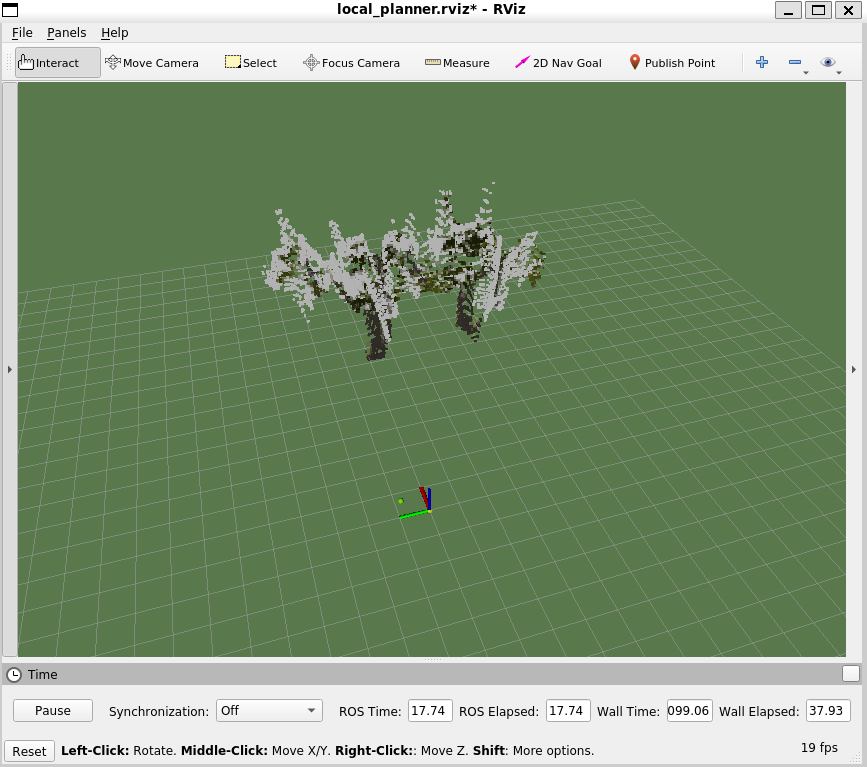
\includegraphics[width=0.4\textwidth]{images/sim_gazebo_points_stereo_voxel.png}}\hfill
    \caption[Punktwolkendarstellung in \textit{rviz}]{Punktwolkendarstellung in \textit{rviz} generiert aus simulierten Bildern}
    \label{fig:sim_gazebo_stereo}
\end{figure}

Zuletzt ist der Transformationsbaum in Bild \ref{fig:sim_gazebo_tftree} abgedruckt. Eine Transformation ist notwendig, um die Position von Objekten (bspw. der Drohne im Raum, Kameras an der Drohne) relativ zu ihrem Bezugspunkt/ Ursprung darzustellen. Die Position der Drohne wird gekennzeichnet durch den Knoten \enquote{fcu} und ist relativ zum Knoten \enquote{local\_origin}. Um alle bekannten Punkte im Raum anpeilen zu können (von einem bekannten Punkt aus), sollten alle Knoten miteinander verknüpft sein. Jedoch besteht der Transformationsbaum hier aus 4 einzelnen Strängen. Dies ist der Konfiguration von \textit{mavros} geschuldet, die wiederrum in \textit{Avoidance} integriert ist. Die Themen \enquote{map} und \enquote{odom} werden von \textit{mavros} zur Navigation genutzt. Die Transformation \enquote{base\_link} wurde in einer neueren Version von \textit{mavros} eingeführt und soll den Mittelpunkt eines Roboters darstellen, wird aber im Projekt nicht genutzt\footnote{\url{https://www.ros.org/reps/rep-0105.html\#base-link}}. Sowohl \textit{mavros} als auch \textit{Avoidance} können mit dem bestehenden Transformationsbaum arbeiten. Wird ein neues Objekt (bspw. Darstellung einer Punktwolke) im Koordinatensystem 
erzeugt, muss auch eine entsprechende Transformation angelegt werden. Für die Tiefenbilder kommt hier das Thema \enquote{camera\_link}, relativ zur Position der Drohne, zum Einsatz.
\begin{figure}[!ht]
    \centering
    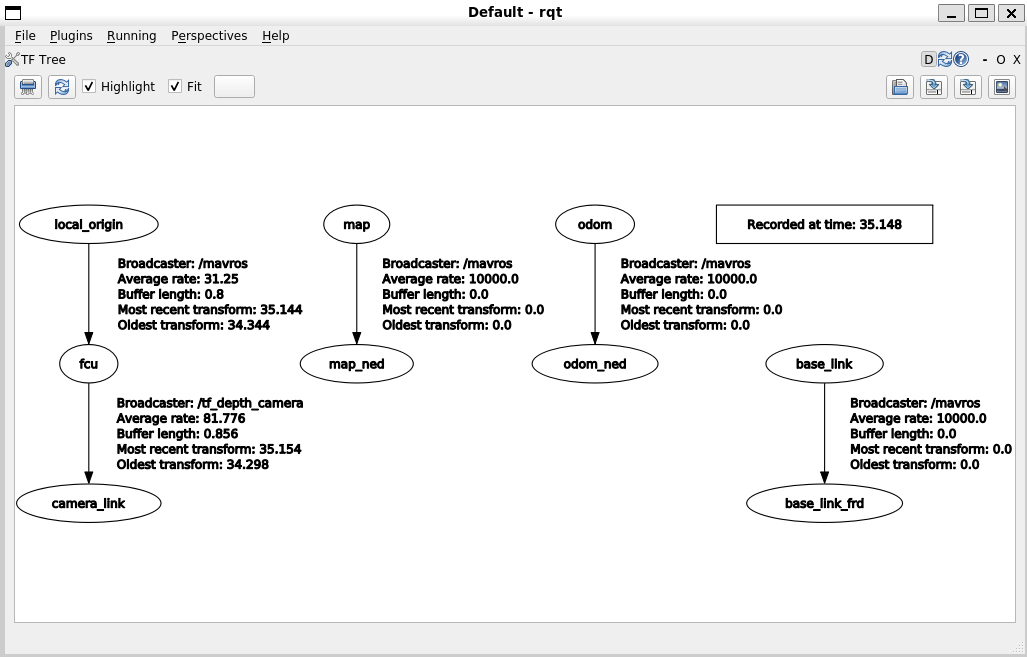
\includegraphics[width=\linewidth]{images/sim_gazebo_tftree.png}
    \caption{Transformationsbaum tftree bei Simulation von \textit{Local Planner}}
    \label{fig:sim_gazebo_tftree}
\end{figure}

\section{Avoidance als Simulation mit Hardware}
Als nächste Stufe der Simulation kommt der Simulator \enquote{AirSim} von Microsoft zum Einsatz. Mit \textit{AirSim} stehen die gleichen Möglichkeiten zur Simulation wie mit \textit{Gazebo} zur Verfügung. Allerdings, kann \textit{AirSim} für das Projekt nur mit einem Windows PC zum verwendet werden. Dadurch ergeben sich Beschränkungen, wodurch \textit{AirSim} keine Verbindung zum simulierten Flugcontroller aufbauen kann. Jedoch kann der reale Flugcontroller wie in \cite[Kapitel 5]{markusreinErweiterungBestehenderDrohnen2023} als \gls{hil}-Simulation betrieben werden. Die Veränderungen im Aufbau für die Simulation sind in Bild \ref{fig:system_sim_airsim} rot markiert, die Funktionen der Bestandteile bleiben die gleichen wie in \cref{chap:sim_gazebo}. Hinzu kommt der Bordcomputer, der eine netzwerkgebundene Kommunikation mit dem Flugcontroller erlaubt und der Knoten \enquote{AirSim-Node}, durch den Bilder aus der Simulation ausgelesen werden können. Dabei entfällt das Zusammenfügen zweier Stereobilder, denn die Simulation liefert direkte Tiefenbilder.

\begin{figure}[!ht]
    \centering
    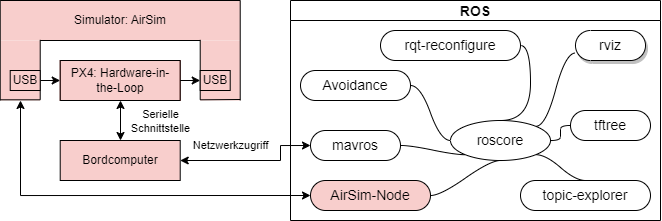
\includegraphics[width=\linewidth]{images/simulation_ros-Page-2.drawio.png}
    \caption[Systemaufbau der Simulation von Avoidance als \gls{hil}-Simulation]{Systemaufbau der Simulation von Avoidance als \gls{hil}-Simulation: Links Simulator (AirSim) und Flugcontroller (\gls{hil}), Rechts Bestandteile des \acrshort{ros}}
    \label{fig:system_sim_airsim}
\end{figure}

Zur Änderung der Funktionalität werden die \textit{Launch-Files} und \enquote{airsim\_ros\_pkgs} (Bibliothek zur Drohnensteuerung im \textit{AirSim}-Simulator) nacheinander angepasst:
\begin{enumerate}
    \item \textit{local\_planner\_stereo.launch}:
    \begin{itemize}
        \item Umbenannt zu \textit{local\_planner\_hitl\_airsim.launch}
        \item Entfernen der Funktion von Disparitätsbildern, da Anwendung keinen ersichtlichen Zweck erfüllt
        \item Unteraufruf von \textit{avoidance\_hitl\_airsim.launch} anstatt \textit{avoidance\_sitl\_stereo.launch}
    \end{itemize}
    \item \textit{avoidance\_sitl\_stereo.launch}:
    \begin{itemize}
        \item Umbenannt zu \textit{avoidance\_hitl\_airsim.launch}
        \item Entfernen der Stereo-Bildverarbeitung, stattdessen Berechnung der Punktwolkendarstellung aus Tiefenbild von \textit{AirSim}
        \item Entfernen der Transformation von \enquote{fcu} auf \enquote{camera\_link}, da Punktwolkendarstellung noch nicht bekannt
        \item Unteraufruf von \textit{avoidance\_hitl\_airsim\_mavros.launch} anstatt \textit{avoidance\_sitl\_mavros.launch}
    \end{itemize}
    \item \textit{avoidance\_sitl\_mavros.launch}:
    \begin{itemize}
        \item Umbenannt zu \textit{avoidance\_hitl\_airsim\_mavros.launch}
        \item Entfernen Startvorgang des \enquote{PX4 SITL} (Software Simulation des Flugcontrollers)
        \item Ändern des Parameters \enquote{fcu\_url} auf lokale IP-Adresse des Onboard-Computers
        \item Ändern des Parameters \enquote{gcs\_url} auf lokale IP-Adresse des Simulations-PC
        \item Entfernen Startvorgang von \textit{Gazebo}
        \item Einfügen Startvorgang der \enquote{AirSim-Node} (Bestandteil der \textit{airsim\_ros\_pkgs}) zur Darstellung eines simulierten Gefährts, dabei noch wichtige Anpassungen: das erzeugte Tiefenbild muss im Untertopic wie die zugehörige \enquote{camera\_info} vorzufinden sein; der Ursprung aller Ortstransformationen, gennant \enquote{world\_frame\_id} wird entsprechend an \textit{local\_origin} angeknüpft
    \end{itemize}
    \item Einstellungen zu \textit{AirSim}:
    \begin{itemize}
        \item Anlegen eines \enquote{vehicle}, hier eine Drohne \textit{PX4} die über USB mit der realen Hardware verbunden ist
        \item Anlegen einer Kamera innerhalb der Drohne, hier vom Typ \enquote{DepthPlanar}, gennant \enquote{mk1}
    \end{itemize}
    \item Einstellungen zu \textit{airsim\_ros\_pkgs}:
    \begin{itemize}
        \item Aufbau einer Verbindung zum Windows-Rechner mit \textit{AirSim}-Simulator
        \item Anhängen des Transformationsbaum von \textit{AirSim} an Transformationsbaum von \textit{mavros} um Transformation der Punktwolke (aus Kamerabild) zur Drohne zu ermöglichen  
        \item Ausgliedern generierter Tiefenbilder aus Transformationsbaum von \textit{AirSim}
        \item Eingliedern generierter Tiefenbilder in Transformationsbaum von \textit{mavros}, dazu wurde die Punktwolke noch entsprechend transformiert, siehe Bild 
    \end{itemize} 
\end{enumerate}

Als Simulation von \textit{AirSim} wurde die \enquote{Blocks}-Umgebung gewählt, eine einfache Welt mit wenigen Objekten. Die Ausgangssituation ist dargestellt im Anhang unter \ref{fig:sim_airsim}. Dabei steht die Drohne vor einem großen Quader. Rechts vom Quader befindet sich eine Kugel.

Probleme die bei der Durchführung durchlaufen wurden, umfassen unter anderem, dass \textit{AirSim} von einem Koordinatensystem im Format \enquote{ENU} (East-North-Up) als die Interpretation der Welt, in der sich die Drohne befindet, ausgeht. Von \textit{mavros} wird die Drohne hingegen im Format \enquote{NED} (North-East-Down) beschrieben. Somit ist das erfasste Kamerabild nicht vor, sondern rechts der Drohne und steht Kopfüber. Die erfasste Punktwolke der Ausgangssituation ist zu sehen in Bild . Anschließende Anpassungen des Transformationsbaums ergeben eine Ansicht wie in . Der finale Transformation ist in Bild  abgebildet.

Das ganze funktioniert so nicht... wer hätts gedacht

\clearpage
    \section{Machbarkeitsstudie Stereokamera mit Raspberry Pi}
Vor der Anschaffung eines Kameramoduls für den Raspberry Pi, soll die Nutzbarkeit bewertet werden.\\
AC:
\begin{itemize}
    \item flüssige Ausgabe von Punktwolke, Avoidance benötigt $10-20$ \gls{fps}
    \item Erfassung großer Gegenstände, kleine Texturen können je nach Kamera und Lichtverhältnissen nicht erfasst werden
    \item Erfassung von Gegenständen im Nahbereich vor der Kamera, weitläufiger Hintergrund kann vernachlässigt werden
\end{itemize}

\acrshort{ros} stellt eine Beispiel-Videoaufnahme mit einer Auflösung von $640x480$ Pixeln und $15$ \gls{fps} Bildwiederholrate bereit, die von 2 Kameras als linke und rechte Perspektive aufgenommen wurde. Diese wird als Referenz für die Tests verwendet.

\paragraph*{Durchführung}
\acrshort{ros} stellt die notwendige Software zur Verfügung. Mit dem Programm \textit{stereo\_image\_proc} können 2 Bilder (Linkes und Rechtes Bild) zu einem Tiefenbild zusammengeführt werden.

Optimierung steht im Kontext hier für eigene Kompilierung mit den C++-Compiler Flags \texttt{-march=native -O3}. Durch diese wird eine Anpassung auf den aktuell verwendeten Prozessor aktiviert. Speziell die Bildverarbeitung mittels OpenCV kann durch parallele Verarbeitung mit sog. Streaming-Befehlssätzen, ähnlich einer Grafikkarte, beschleunigt werden.  
\begin{table}[!ht]
    \label{tab:bench_stereo_image_proc}
    \caption{Benchmark zum Programm \textit{stereo\_image\_proc} auf dem \gls{rpi}}
    \begin{tabularx}{\textwidth}{>{\raggedright\arraybackslash}X|>{\raggedright\arraybackslash}X|>{\raggedright\arraybackslash}X}
    Versuch &   Auflösung normal (640x480)    &   Auflösung halbiert (320x240)\\
    \hline
    Standard Packete    &   6.3 &   14.7\\
    \hline
    Optimiertes OpenCV  &   6.9 &   14.7\\
    \hline
    Optimiertes OpenCV,\newline vision\_opencv und image\_pipeline & 6.7 & 14.6\\
    \end{tabularx}
\end{table}

    \appendix
    \chapter{Anhang}

\begin{figure}[!ht]
    \centering
    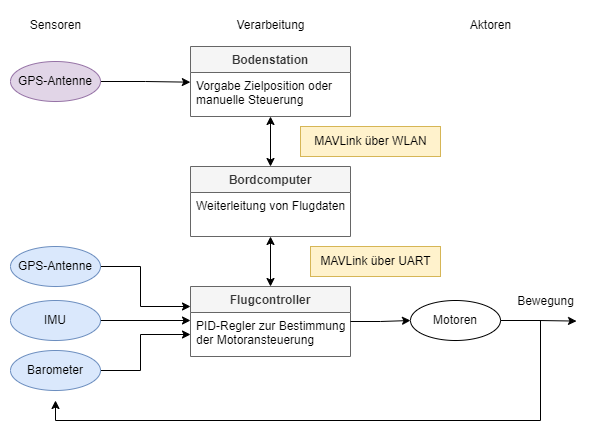
\includegraphics[width=\linewidth]{images/001_vereinfacht-Page-3_default.drawio.png}
    % oder mehrere Bilder, dann aber IMMER MIT \hfill !!!!
    %\subfloat[Bild 1]{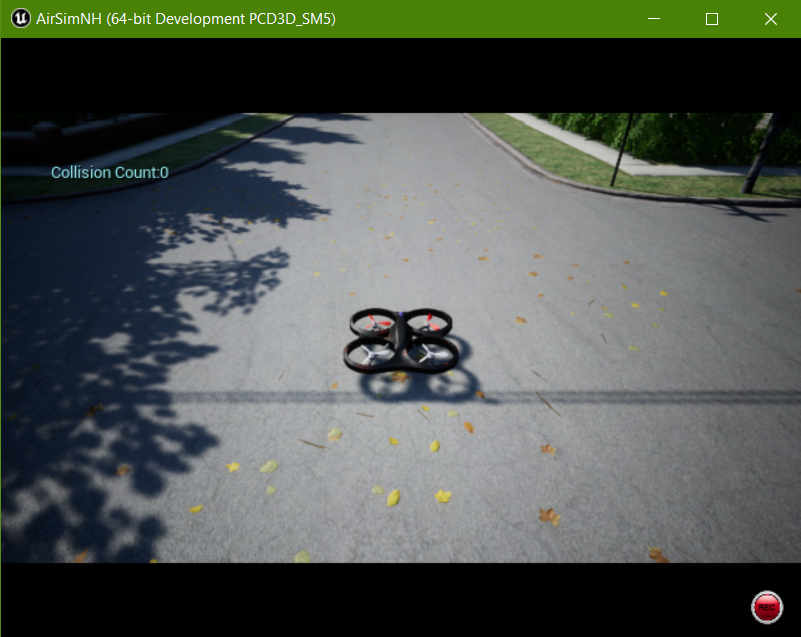
\includegraphics[width=0.4\textwidth]{images/sim_initial.png}}\hfill
    %\subfloat[Bild 2]{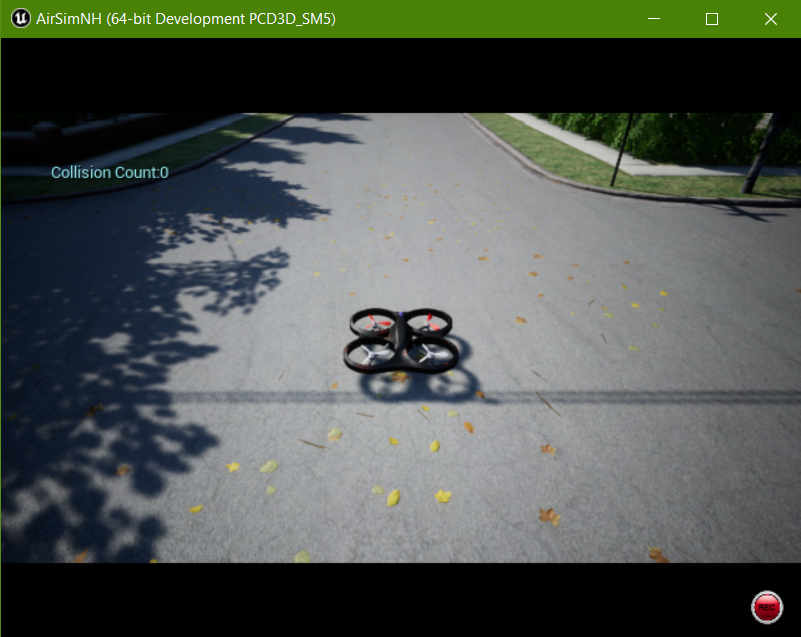
\includegraphics[width=0.4\textwidth]{images/sim_initial.png}}\hfill
    \caption[Beschreibung des Systems Drohne-Bodenstation]{Beschreibung des Systems Drohne-Bodenstation: Grau hinterlegt die Bestandteile aus Tabelle \ref{tab:system_intro}; Gelb hinterlegt das jeweilige Kommunikationsprotokoll; Blau hinterlegt vorhandene Sensoren; Lila hinterlegt optionale Sensoren}
    \label{fig:system_intro}
\end{figure}

\begin{figure}[!ht]
    \centering
    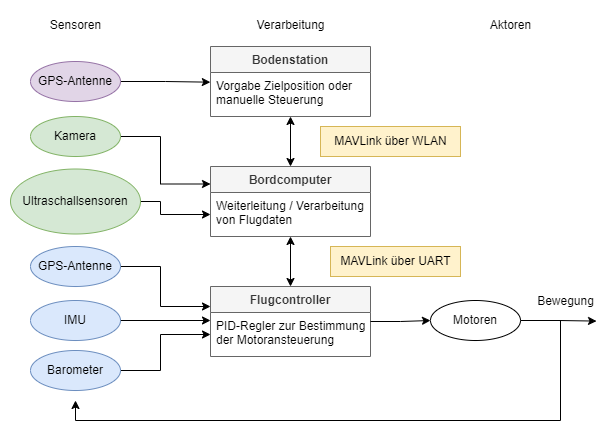
\includegraphics[width=\linewidth]{images/001_vereinfacht-Page-3_erweitert.drawio.png}
    \caption[Beschreibung des erweiterten Systems Drohne-Bodenstation]{Beschreibung des erweiterten Systems Drohne-Bodenstation: Grün hinterlegt neu vorgesehene Sensoren}
    \label{fig:system_added_sensors}
\end{figure}

\begin{figure}[!ht]
    \centering
    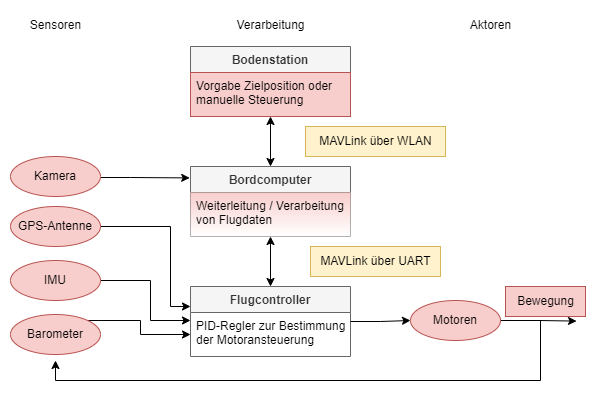
\includegraphics[width=\linewidth]{images/001_vereinfacht-Page-3_simuliert.drawio.png}
    \caption[Beschreibung des Systems zur Simulation HIL]{Beschreibung des Systems zur Simulation HIL: Hell-rot dargestellt die von der Simulation übernommenen Aufgaben}
    \label{fig:system_sim}
\end{figure}

\begin{figure}[!ht]
    \centering
    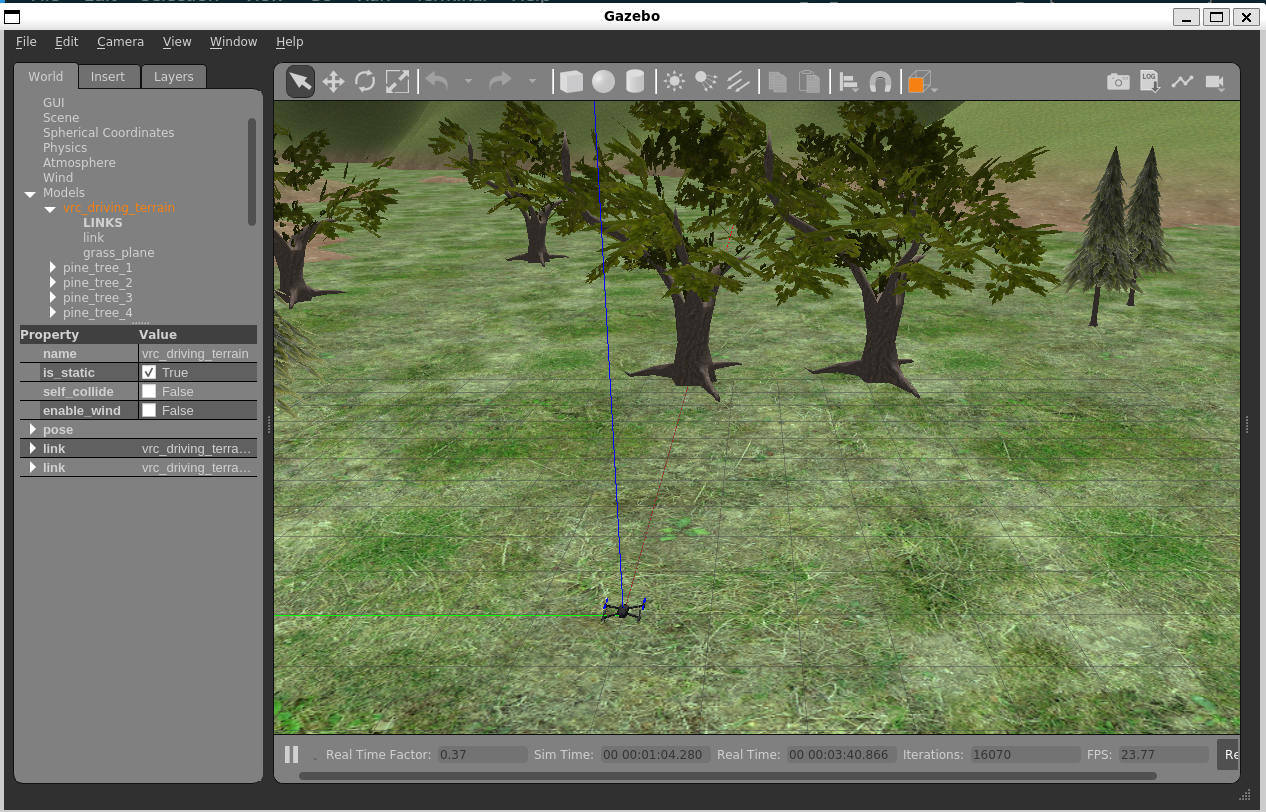
\includegraphics[width=\linewidth]{images/sim_gazebo.png}
    \caption[Ansicht Gazebo Simulator]{Erste Ansicht von Gazebo bei der Simulation von Avoidance: Relativ klein im Vordergrund die simulierte Drohne mit Koordinatenachsen (Rot, Grün, Blau), im Hintergrund die Welt mit Bäumen, auf linker Seite ein Konfigurationsmenü von Gazebo}
    \label{fig:sim_gazebo}
\end{figure}

\begin{figure}[!ht]
    \centering
    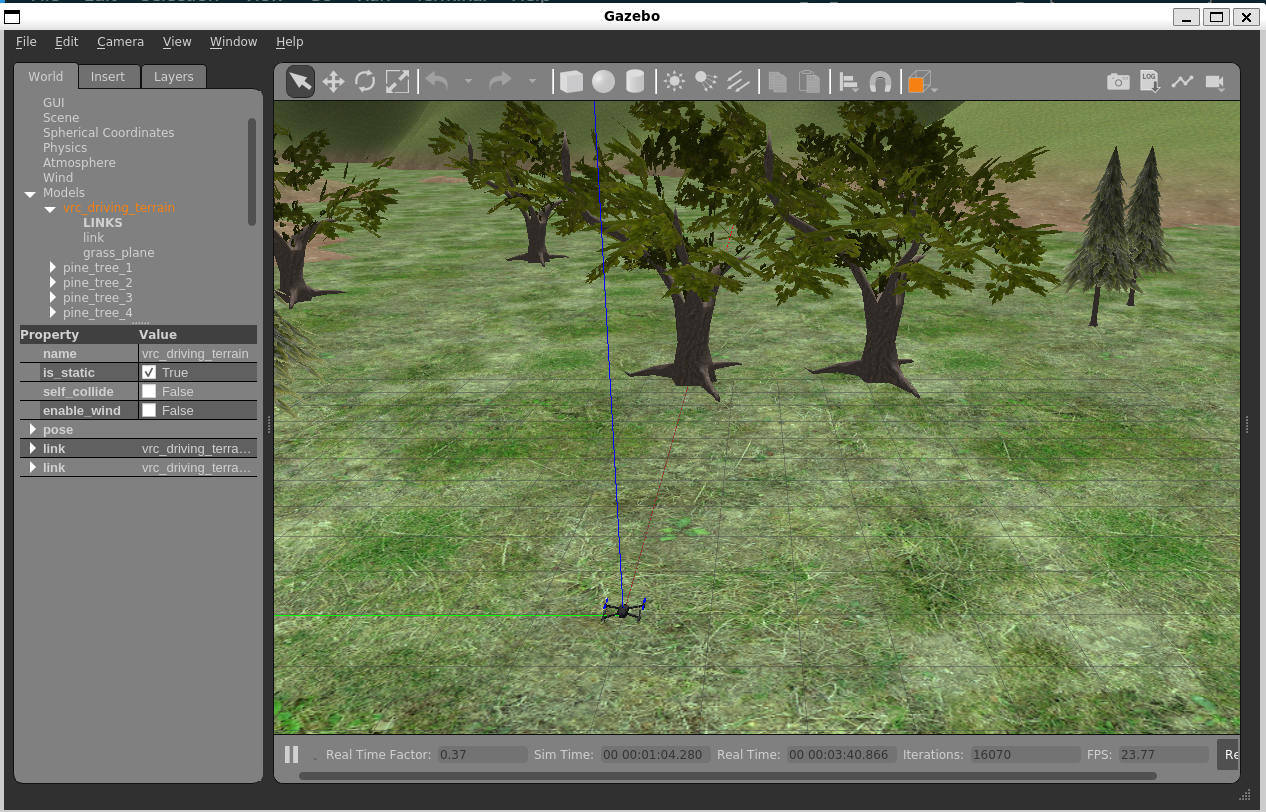
\includegraphics[width=\linewidth]{images/sim_gazebo.png}
    \caption[Ansicht Gazebo Simulator]{Erste Ansicht von AirSim bei der Blocks-Simulation: im Vordergrund die simulierte Drohne, im Hintergrund ein großer Quader und eine Kugel}
    \label{fig:sim_airsim}
\end{figure}

    % ********************************************************************
    % End of contents
    % ********************************************************************

    \backmatter
    \cleardoublepage
    \printbibliography

    \cleardoublepage
    \listoffigures
    \cleardoublepage
    \listoftables
    \cleardoublepage
    \printnoidxglossaries
    % Appendix, if needed:


\end{document}